\documentclass[a4paper, 12pt]{report}

%%%%%%%%%%%%
% Packages %
%%%%%%%%%%%%

\usepackage[spanish]{babel}
\usepackage{packages/sleek}
\usepackage{packages/sleek-title}
\usepackage{packages/sleek-theorems}
\usepackage{packages/sleek-listings}
\usepackage{dirtree}
\usepackage{tikz}
\usepackage{pgfplots}
\usepackage{pgfplotstable}
\usepackage{tikz}
\usetikzlibrary{automata} % Carga la librería automata




%%%%%%%%%%%%%%
% Title-page %
%%%%%%%%%%%%%%

\logo{./resources/pdf/logo.pdf}
\institute{Universidad Politécnica de Cartagena}
\faculty{Ingeniería Telemática}
%\department{Department of Anything but Psychology}
\title{Conexión Cliente-Servidor mediante sockets en Java}
\subtitle{Trabajo de prácticas de sistemas distribuidos }
\author{\textit{Autores}\\\textsc{Álvaro Herández Riquelme}\\ y \textsc{André Yermak Naumenko}}
%\supervisor{Linus \textsc{Torvalds}}
%\context{A long time ago in a galaxy far, far away...}
\date{\today}

%%%%%%%%%%%%%%%%
% Bibliography %
%%%%%%%%%%%%%%%%

\addbibresource{./resources/bib/references.bib}

%%%%%%%%%%
% Macros %
%%%%%%%%%%

\def\tbs{\textbackslash}

%%%%%%%%%%%%
% Document %
%%%%%%%%%%%%

\begin{document}
\maketitle
\romantableofcontents

\newpage

\chapter{Introducción}

En este documento se presenta el trabajo realizado en la asignatura de sistemas distribuidos, en el cual se ha
implementado un sistema de transferencia de archivos entre un cliente y un servidor mediante sockets en Java.
Se ha elegido el uso de sockets para la comunicación entre el cliente y el servidor, ya que lo consideramos una
forma más sencilla y eficiente de implementar lo que se pide en estre trabajo.

\section{Estructura del proyecto}

La estructura del proyecto se basa mayoritariamente alrededor de \textbf{la máquina de estados} que hemos
diseñado para éste, siendo de gran importancia el contexto que tenga el programa en todo momento, ya sea
cliente, servidor, o sistema. Con esta implementación, se ha conseguido que en la misma ejecución del programa se pueda pasar de cliente a servidor en un determinado momento si es que el usuario lo desea.
%
%    \begin{figure}[htb]
%        \centering
%        \begin{tikzpicture}[]
%            \node[state] (s1) {Sistema};
%            \node[state, below right of=s1] (s2) {Cliente};
%            \node[state, below left of=s1] (s3) {Servidor};

%            \draw
%            (s1) edge[bend left]    (s2)
%            (s1) edge[bend right]   (s3)
%            (s2) edge[bend left]    (s1)
%            (s3) edge[bend right]   (s1);
%        \end{tikzpicture}
%        \caption{Máquina de estados diseñada para el proyecto.}
%        \label{fig:diagrama}
%    \end{figure}

\begin{figure}[H]
	\centering
	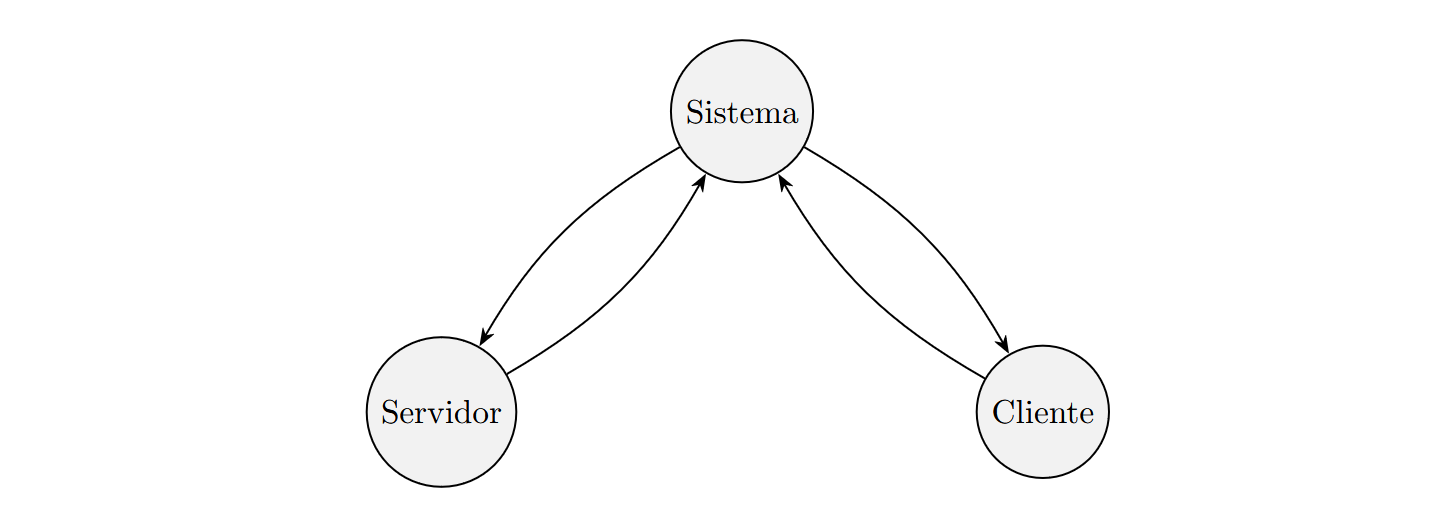
\includegraphics[scale=0.40]{resources/img/diagrama.png}
	\caption{Máquina de estados diseñada para el proyecto.}
	\label{fig:main}
\end{figure}


Como podemos apreciar en la figura \ref{fig:main}, tras arrancar el programa estamos en el contexto de Sistema, éste puede pasar de un estado a otro en cualquier momento, sin permitir que el cliente pase a servidor de forma directa ya que esto conllevaría a graves errores.
Por otro lado, la estructura de archivos finalmente quedará organizada de la siguiente manera:

\newpage
\begin{figure}
\dirtree{%
	.1 .
	.2 FileSystem.java.
	.2 Main.java.
	.2 SystemContextHandler.java.
	.2 client.
	.3 ClientContextHandler.java.
	.3 ClientMain.java.
	.3 ClientUtils.java.
	.3 SimpleClient.java.
	.2 common.
	.3 CommandMessage.java.
	.3 ConsoleGUI.java.
	.3 Const.java.
	.3 Context.java.
	.3 ContextCommandHandler.java.
	.3 ContextManager.java.
	.3 ContextObserver.java.
	.3 Header.java.
	.3 Utils.java.
	.2 META-INF.
	.3 MANIFEST.MF.
	.2 server.
	.3 ConcurrentServer.java.
	.3 SimpleServer.java.
	.3 ServerCommandProcess.java.
	.3 ServerContextHandler.java.
	.3 ServerMain.java.
}
\captionof{table}{Estructura de archivos del proyecto.}
\end{figure}

\chapter{Filetransfer}
\section{Uso del programa}
varo
\section{Main.java}
Main inicializa FileSystem.
\section{FileSystem.java}
FileSystem es la encargada de inicializarlo todo, la interfaz gráfica (si es que el usuario no ha puesto como argumento de entrada \texttt{--nogui} o le ha dado doble click al .jar), las carpetas de gestión de archivos y el config.yml, que permite al usuario dejar argumentos de carga preestablecidos, de tal forma que no tenga que escribirlos cada vez que quiera iniciar el programa, los argumentos que se pueden guardar son:
Puerto de servidor, número máximo de conexiones que un servidor puede aceptar y dirección IP a la que el cliente se conectará.
Y por último inicializa la lectura por consola.
\section{SystemContextHandler.java}
SystemContextHandler es el primer contexto que instancia el usuario al arrancar el programa. 
Para ver los comandos disponibles hay que escribir en consola alguno de los siguientes comandos: 
\texttt{?}, \texttt{--help} o \texttt{-h}, que devolverá por pantalla los comandos disponibles que son 
en el contexto del sistema \texttt{--client} y \texttt{--server} con sus argumentos opcionales.


\chapter{common}

La carpeta common es la que contiene las clases que son compartidas por los 3 contextos. En ella podemos encontrar clases como los serializadores de objetos que son, el Header, CloseMessage,TextMessage y CommandMessage. También podemos encontrar las interfaces y constantes para gestionar los estados del programa entre otros.
\section{CommandMessage.java}

Es la clase encargada de crear todos los comandos y que además puedan esos comandos puedan construirse con argumentos y payload en el objeto desde la subclase Builder
Comandos disponibles:

\begin{itemize}
	\item \texttt{FILE\_UPLOAD}
	\item \texttt{FILE\_DOWNLOAD}
	\item \texttt{FILE\_RENAME}
	\item \texttt{DIRECTORY\_CREATE}
	\item \texttt{DIRECTORY\_LIST}
	\item \texttt{DIRECTORY\_LOCATION}
	\item \texttt{FILE\_DELETE}
	\item \texttt{DIRECTORY\_OPEN}
	\item \texttt{ECHO\_FILE}
	\item \texttt{CON\_CHECK}
\end{itemize}

\section{ConsoleGUI.java}
Se ha creado una interfaz gráfica opcional (si el usuario al arrancar el programa desde la consola con el argumento --nogui no se iniciará la consola) se encarga de redirigir simplemente todos los mensajes en consola al Textarea, la implementación ha sido inspirada y adaptada de Stackoverflow. \cite{console-output-to-textarea}
\section{Const.java}
En FileSystem, hay muchos valores que son constantes y se recurren muy amenudo, por lo que se ha decidido crear una clase estática que contenga todas las constantes que se usan en el programa.
\section{Context.java}
Es un enum que contiene los estados posibles del programa.
\section{ContextCommandHandler.java}
Una interfaz para todos los contextos que manejan comandos.
\section{ContextManager.java}
Es la clase encargada de gestionar los contextos, y poder alternar entre ellos sin problemas.
\section{ContextObserver.java}
Una interfaz necesaria principalmente para la consola gráfica la cual necesita ser notificada de los cambios de contexto.
\section{Header.java}
Es la clase que le da cabecera a todos los objetos serializables, en nuestro caso se ha quedado como vestigio por usar serialización automática.
\section{Utils.java}
Esta clase estaba destinada a tener métodos útiles, pero finalmente se ha empleado simplemente para obtener las direcciones IP tanto pública como privada del servidor.	

\chapter{client}
\section{ClientMain.java}

El \textbf{ClientMain} es la primera instancia que se crea al hacer el cliente. En el momento que en la consola se elige el contexto con --client, se crea una instancia principal que gestiona el puerto y el host que se le envía, e intenta iniciar una nueva conexión. En caso de que exista un servidor escuchando en el host y puerto seleccionado, se creará un \textbf{socket}, una clase de \textbf{SimpleClient} que hará las operaciones del cliente, y se le pasará esta instancia de \textbf{SimpleClient} al ContextHandler, que hemos visto que manejará el puente entre los \textbf{tres contextos posibles.}
Como se ha comentado, las operaciones principales pasan a ser parte del \textbf{simpleClient}

\section{SimpleClient.java}

Al iniciar un SimpleClient, hay operaciones iniciales que se deben hacer para mantener un contexto y un estado del programa. Una vez creada la instancia, se ejecuta la función \textbf{setState} que cambia el estado al enum de estado de conexión \textbf{CONNECTED} si la conexión ha sido correcta. Esto ayudará a comunicarse con el servidor y que se pueda saber su estado de conexión.
A su vez, al inicio igualmente, se comprueba si la carpeta \textbf{Storage} está creada, ya que será la raíz principal de los directorios a compartir o descargar. Se llama a la función \textbf{EnsureDirectoryStructure} y si no está creada la creará mediante la clase Files del paquete java.nio.

Una vez se ha inicializado y creados los sockets, se procede al recibimiento y envío de objetos. Para ello, Se tienen un \textbf{ObjectOutputStream y ObjectInputStream} que vienen de sus respectivos streams, que servirán para el envío y recepción de objetos.

Para el recibimiento de mensajes, se maneja con dos métodos: \textbf{recieveMessages()} y \textbf{handleCommandResponse()}. Principalmente en el bucle, se llama desde un hilo a \textbf{recieveMessages}, cuya finalidad será con el objeto \textbf{ObjectInputStream} creado, se llama a su método \textbf{readObject}, que nos devolverá el objeto cuando se nos envíe desde el otro extremo, que en este caso será el servidor.

De forma similar a la que hacemos en clase, al recibir el objeto se hará un \textbf{casting} que compara de qué tipo es el objeto que previamente ha enviado el servidor. Se comparará si es un objeto de tipo \textbf{CommandMessage} o un \textbf{String}. No se contempla un tipo distinto de objeto. El \textbf{String} vendrá de parte del servidor si éste nos quiere enviar un mensaje, por lo que simplemente imprimirá por pantalla lo que se recibe.

En caso de que se haya recibido un \textbf{CommandMessage}, se llamará a \textbf{handleCommandResponse}, como el servidor sabemos que sólo nos enviará un commandmessage en caso de que sea un archivo, se desempaquetará el payload de bytes que está en el comando y se escribirá en la carpeta seleccionada. No se contempla que el servidor use el CommandMessage de otra forma, pues para eso se usarán Strings.

\section{ClientContextHandler.java}
varo

\section{ClientUtils.java}
varo

\chapter{server}

\section{ServerMain.java}

Al inicio del contexto en el servidor, se crea una instancia de \text{ServerMain}, que actúa como el punto de
entrada principal para iniciar un servidor de transferencia de archivos. La clase extiende ContextManager,
por lo que hereda funcionalidades relacionadas con la gestión del contexto. Al instanciarse, ServerMain recibe
un puerto como parámetro y utiliza métodos de la clase Utils (getPublicIP() y getPrivateIP())
para obtener tanto la dirección IP pública como la privada del
servidor. Estas direcciones IP se almacenan en variables de instancia y se muestran por consola cuando el servidor se inicia.

\textbf{El método start}:

Es el encargado de iniciar el servidor. Primero, imprime un mensaje
indicando que el servidor ha comenzado a escuchar en el puerto
especificado, junto con las direcciones IP pública y privada. Luego,
crea una instancia de ConcurrentServer, pasando el puerto y la propia instancia de ServerMain (que actúa como ContextManager) como argumentos. Finalmente, llama al método run() de ConcurrentServer,
lo que inicia el servidor concurrente y comienza a aceptar conexiones
de clientes. Este diseño permite que el servidor maneje múltiples
conexiones de manera eficiente, utilizando un pool de hilos para
gestionar cada cliente de forma independiente.



\section{ConcurrentServer.java}

El concurrentserver, cuyo nombre viene dado por las prácticas aunque se haya modificado, manejará múltiples
conexiones de clientes utilizando un pool de hilos. Cuando el servidor se inicia, escucha en un puerto
específico y declara un \texttt{ExecutorService}  con un número fijo de hilos definido por
\texttt{Const.MAX\_THREADS}. El servidor entra en un bucle infinito donde espera conexiones de clientes. Cada
vez que un cliente se conecta, se crea obtiene un \texttt{Socket} que
representa la conexión con ese cliente y muestra la dirección del cliente
conectado. Para manejar la conexión, el servidor crea un nuevo hilo en el pool, donde se instancia un
objeto \texttt{SimpleServer} pasándole el socket del cliente y se llama al método `run()`. Este método es el
gestionará la comunicación con el cliente. De esta forma el servidor atiende a varios
clientes de manera simultánea mediante los hilos.

\section{SimpleServer.java}

Una vez hecho el hilo y formado el socket de conexión, se necesita una forma de comunicación entre los procesos. Cada conexión del servidor con un cliente distinto tendrá una instancia independiente de \textbf{SimpleServer}, donde se implementa el manejo de objetos tanto de \textbf{input} como de \textbf{output}.

\textbf{Recepción del mensaje serializado}

Al iniciar la instancia de SimpleServer, también se creará un \textbf{ObjectInputStream}, leído del \textbf{InputStream}, que deserializa y crea el objeto de lo enviado anteriormente mediante OutputStream.
En este caso, como es el cliente el único que le envía al servidor, haremos un \textbf{casting} del objeto recibido, para comprobar que efectivamente es un \textbf{CommandMessage}, el único objeto que debe recibir el servidor de parte del cliente. Una vez comprobado si pertenece a la clase correcta, si el mensaje pidió una descarga de archivo se busca en el \textbf{Path correspondiente} si el archivo existe, y si existe se empaquetan los bytes y se envía la respuesta del archivo pedido.

En caso de que el objeto del servidor sea un \textbf{CommandMessage} y no sea una petición de descarga, se llamará al método \textbf{processCommand} de la clase \textbf{ServerCommandProcess} añadiendo de argumentos el comando y el path, que procesará una respuesta según el comando que haya sido. Una vez recibida la respuesta que le debe pasar se envía mediante el \textbf{ObjectOutputStream}

\section{ServerCommandProcess.java}

El ServerCommandProcess, es el encargado de procesar los objetos \textbf{CommandMessage} que recibe el
servidor, y actuar en consecuencia. Cada comando requiere una función propia, y al optar
por hacerlo con un enfoque distinto al de clase, donde cada comando podría ser una clase distinta y que cada
función se ejecute según el objeto, se ha hecho un \textbf{hashmap} que contiene las funciones que se ejecutarán
según el comando que se reciba.

Todas las funciones que se ejecutan en el hashmap, reciben un objeto de tipo \textbf{commandMessage},
que viene de \textbf{SimpleServer}. Ya habiendo pasado las validaciones tanto de tipado (el casting),
como de argumentos (En la parte del cliente). Cada función del hashmap también recibe un objeto de tipo
\textbf{Path}, del paquete de java.nio, que será el directorio en el que se ejecutará el comando, el cual se
procesa al inicio de la clase. Este path es una combinación del basepath, donde se encuentra el storage, y el
clientpath, que será el directorio en el el servidor entiende que se encuentra el cliente.
Se tiene en cuenta que el cliente no pueda salir del directorio base.

Cada función opera de forma distinta, según el comando, aunque la mayoría son operaciones que nos permite ejecutar el paquete \textbf{java.nio}

\section{ServerContextHandler.java}

El serverContextHandler hace función similar que el clientContextHandler, pero en menor medida, ya que el
dispositivo que actúa como servidor no tiene que enviar muchos comandos, por lo que tiene comandos basicos como
--close o --help, para cerrar u obtener ayuda de los posibles comandos del servidor. No está pensado para interactuar mucho, su finalidad es recibir peticiones del cliente y procesarlas.

\printbibliography
\end{document}
